\documentclass[fleqn]{jbook}
\usepackage{physpub}

\begin{document}
\begin{question}{教育 数学}{}
\begin{subquestions}

\SubQuestion
 関数$y(x)$に対する次の常微分方程式について以下の設問に答えよ。
   \[\frac{1}{x^2}\frac{d}{dx}\left(x^2\frac{dy}{dx}\right)=-y^n\]
ただし、$y(0)=1$,$\displaystyle{
\left.\frac{dy}{dx}\right|_{x=0}=0}$ とする。
\begin{subsubquestions}
\SubSubQuestion
$n=0$の場合の解を求めよ。
\SubSubQuestion 
$y=\displaystyle{\frac{z}{x}}$とおいて、$z$に対する微分方程式を導き、
$n=1$の場合の解を求めよ。
\SubSubQuestion
$n=0,n=1$の場合のほかに、ある整数$n$に対して次の形の解
    \[y=(1+ax^2)^m\]
が存在することが知られている。その整数$n$と、定数$m$、$a$を求めよ。
\SubSubQuestion
$x=0$の近傍の解を$x$に関するべき級数に展開し、$x^4$の項まで求めよ。
\end{subsubquestions}

\SubQuestion
3行3列の行列に関して以下の設問に答えよ。
\[ A=\left(\begin{array}{rrr}
            1 & 0 & 2 \\
            0 & 1 & 2 \\
            2 & 2 & -1
          \end{array}\right)\]

\begin{subsubquestions}
\SubSubQuestion
$A$の固有値と固有ベクトルを求めよ。
\SubSubQuestion
行列に関する方程式
 \[A^3+aA^2+bA+cE=0 \]
の係数a,b,cを求めよ。但し$E$は3行3列の単位行列、$0$は零行列である。
この結果を用いて行列
   \[A^5-6A^3-4A^2+18E \]
を計算せよ。
\SubSubQuestion
 3次元ベクトル空間$R^3$のベクトル$\vec{x}$で、$R^3$のあるベクトル
$\vec{y}$を用いて
 \[ \vec{x}=(A-E)\vec{y} \]
と表すことのできないものの一般形を求めよ。
\end{subsubquestions}

\SubQuestion
1辺の長さaの正三角形で構成される正20面体の体積を以下の手順に従って求めよ。
図1は、正20面体を一つの頂点Aと中心Oを通る直線の方向から見た時の平面図
であり、図2は、その直線と一辺ABを含む平面で切った時の断面図である。
なお断面図には正20面体の内接球も破線で示してある。
\begin{subsubquestions}
\SubSubQuestion
恒等式$(\cos\theta+{ i}\sin\theta)^5=\cos5\theta+{ i}\sin5\theta$
を利用して、$\cos5\theta$を$\cos\theta$の多項式で表せ。ただし$i$は
虚数単位である。
\SubSubQuestion
 上の結果を利用して、$\displaystyle{\cos\left(
\frac{\pi}{5}\right)}$の値を求めよ。
\SubSubQuestion
 正20面体に内接する球の半径を求めよ。また内接点はどの様な点であるか。
\SubSubQuestion
 正20面体の体積を求めよ。

\parbox[t]{80mm}{
\begin{center}
%
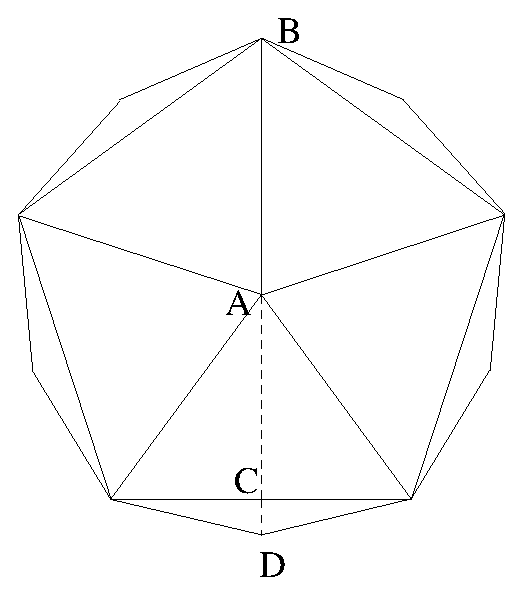
\includegraphics[clip,height=48mm,width=42mm]{1992math-1.eps}

図1
\end{center}
}\parbox[t]{80mm}{
\begin{center}
%
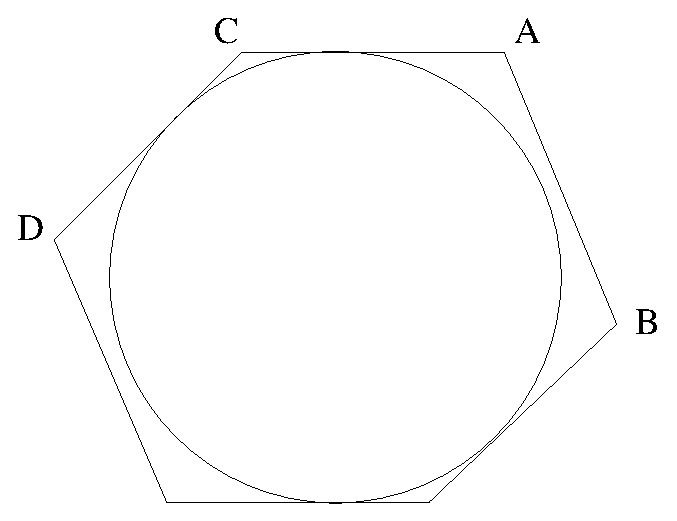
\includegraphics[clip,height=42mm,width=55mm]{1992math-2.eps}

図2
\end{center}
}
\end{subsubquestions}
\end{subquestions}
\end{question}
\begin{answer}{教育 数学}{}
\begin{subanswers}
\SubAnswer
  
\begin{subsubanswers}
\SubSubAnswer
  $\displaystyle{u=x^2\frac{dy}{dx}}$として、もとの方程式を書き直すと、
\[\frac{du}{dx}=-x^2\]
となる。これと、$u(0)=0$から、
\[u=-\frac{x^3}{3}  \qquad \Yueni \frac{dy}{dx}=-\frac{x}{3} \]
これを解いて、
\[y=1-\frac{x^2}{6} \]

\SubSubAnswer
  まず、
\[\frac{dy}{dx}=\frac{d}{dx}\left(\frac{z}{x}\right)
=-\frac{z}{x^2}+\frac{1}{x}\frac{dz}{dx} \]
\[
\frac{1}{x^2}\frac{d}{dx}\left(x^2\frac{dy}{dx}\right)
=\frac{1}{x^2}\frac{d}{dx}\left(-z+x\frac{dz}{dx}\right)
=\frac{1}{x^2}\left(-\frac{dz}{dx}+\frac{dz}{dx}+x\frac{d^2z}{dx^2}
\right) 
=\frac{1}{x}\frac{d^2z}{dx^2}
\]
よって、$z$に対する微分方程式は以下のようになる。
\[\frac{1}{x}\frac{d^2z}{dx^2}=-\left(\frac{z}{x}\right)^n\]

$n=1$のときは、
\[\frac{d^2z}{dx^2}=-z\]
と表される。この一般解は、$A,B$を任意定数として、
\[z=Ae^{ix}+Be^{-ix} \qquad \Yueni y=\frac{z}{x}=\frac{1}{x}\left(Ae^{ix}+Be^{-ix}\right)\]
このうち初期条件を満たすものとして、
\[y=\frac{\sin x}{x} \]

\SubSubAnswer
 $y=(1+ax^2)^m$をもとの方程式に代入して、
\begin{eqnarray*}
\frac{1}{x^2}\frac{d}{dx}\left(x^2\frac{dy}{dx}\right)
&=&\frac{1}{x^2}\frac{d}{dx}\left(2amx^3(1+ax^2)^{m-1}\right) \\
&=&(1+ax^2)^{m-2}\left(6am(1+ax^2)+4a^2m(m-1)x^2\right)  \\
&=&-(1+ax^2)^{mn}
\end{eqnarray*}
が得られる。両辺$(1+ax^2)^{m-2}$で割ると、
\[6am+(4m^2+2m)a^2x^2=-(1+ax^2)^{mn-m+2}\]
となる。
$x=0$で等式が成り立つためには、
\begin{equation}
6am=-1 \eqname{5m1-1}
\end{equation}
が必要である。これから、$a\neq0,m\neq0$が必要であることが言える。

次に$x^2$の項の係数が等しいことより、
\begin{eqnarray}
a^2(4m^2+2m)&=&0 \eqname{5m1-2}\\
mn-m+2&=&0 \eqname{5m1-3}
\end{eqnarray}
または、
\begin{eqnarray}
a^2(4m^2+2m)&=&-a \eqname{5m1-4}\\
mn-m+2&=&1 \eqname{5m1-5}
\end{eqnarray}
がいえる。まず、\eqhref{5m1-2},\eqhref{5m1-3}について考えると、
$a\neq0,m\neq0$と\eqhref{5m1-2}をあわせて、$m=-1/2$がいえる。これと、
\eqhref{5m1-3},\eqhref{5m1-1}から、$a=1/3,n=5$となる。これは、確かにもとの方程式
の解となっている。

次に、\eqhref{5m1-4},\eqhref{5m1-5}について考えると、\eqhref{5m1-4},\eqhref{5m1-1}から、$2m+1=3$、すなわち、$m=1$が言える。\eqhref{5m1-1},\eqhref{5m1-5}にこの結果を代入して、
$a=-1/6,n=0$が得られるが、これは、$n\neq0$であることに反するので
求める解ではない。

以上まとめて、$n=5,m=-1/2,a=1/3$である。

\SubSubAnswer
 初期条件を満たす$y$の4次までの展開式として、
\[y=1+a_2x^2+a_3x^3+a_4x^4+O(x^5) \]
をとる。これを方程式の左辺に代入して、
\begin{eqnarray*}
\frac{1}{x^2}\frac{d}{dx}\left(x^2\frac{dy}{dx}\right)
	&=&\frac{1}{x^2}\frac{d}{dx}\left(2a_2x^3+3a_3x^4+4a_4x^5+O(x^6)\right)\\
	&=&6a_2+12a_3x+20a_4x^2+O(x^3)
\end{eqnarray*}
となる。これから、まず$a_2=-1/6$であることがわかる。
また、右辺についての展開は、$x^2$の項までとれば良く、
\[\left(1-\frac{1}{6}x^2+O(x^3)\right)^n=1-\frac{n}{6}x^2+O(x^3)\]
と左辺の展開を比べて、$a_3=0,a_4=\displaystyle{\frac{n}{120}}$
が得られる。

以上まとめて、4次までの$y$の展開として、
\[y=1-\frac{1}{6}x^2+\frac{n}{120}x^4+\cdots\]
が得られる。
\end{subsubanswers}

\SubAnswer

\def\DET1{
      \left|\begin{array}{ccc}
            1-\lambda & 0 & 2 \\
            0 & 1-\lambda & 2 \\
            2 & 2 & -1-\lambda
      \end{array}\right|
}
\def\MATa{
          \left(\begin{array}{ccc}
            1 & 0 & 2 \\
            0 & 1 & 2 \\
            2 & 2 & -1
          \end{array}\right)
}
\def\MATba{
            \left(\begin{array}{ccc}
                3 & 0 & 0 \\
                0 & -3 & 0 \\
                0 & 0 & 1
            \end{array}\right)
}
\def\MATbb{
            \left(\begin{array}{ccc}
                3^3 & 0 & 0 \\
                0 & (-3)^3 & 0 \\
                0 & 0 & 1^3
            \end{array}\right)
}
\def\MATbc{
            \left(\begin{array}{ccc}
                27 & 0 & 0 \\
                0 & -27 & 0 \\
                0 & 0 & 1
            \end{array}\right)
}
\def\EQNba{
            \left\{\begin{array}{lllll}
                27 & +9a & +3b & +c & =0 \\
                -27 & +9a & -3b & +c & =0 \\
                1 & +a & +b & +c & =0
            \end{array}\right.
}
\def\EQNbb{
            \left\{\begin{array}{lllll}
                A^5 & = & A^4 & +9A^3 & -9A^2\\
                A^4 & = & A^3 & +9A^2 & -9A
            \end{array}\right.
}
\def\MATbd{
            \left(\begin{array}{ccc}
                9 & 0 & 54 \\
                0 & 9 & 54 \\
                54 & 54 & -45
            \end{array}\right)
}
\def\MATbb{
            \left(\begin{array}{ccc}
                3^3 & 0 & 0 \\
                0 & (-3)^3 & 0 \\
                0 & 0 & 1^3
            \end{array}\right)
}
\def\MATbc{
            \left(\begin{array}{ccc}
                27 & 0 & 0 \\
                0 & -27 & 0 \\
                0 & 0 & 1
            \end{array}\right)
}
\def\EQNba{
            \left\{\begin{array}{lllll}
                27 & +9a & +3b & +c & =0 \\
                -27 & +9a & -3b & +c & =0 \\
                1 & +a & +b & +c & =0
            \end{array}\right.
}
\def\EQNbb{
            \left\{\begin{array}{lllll}
                A^5 & = & A^4 & +9A^3 & -9A^2\\
                A^4 & = & A^3 & +9A^2 & -9A
            \end{array}\right.
}
\def\MATbd{
            \left(\begin{array}{ccc}
                9 & 0 & 54 \\
                0 & 9 & 54 \\
                54 & 54 & -45
            \end{array}\right)
}
\def\MATca{
            \left(\begin{array}{ccc}
                0 & 0 & 2 \\
                0 & 0 & 2 \\
                2 & 2 & -2
            \end{array}\right)
}
\begin{subsubanswers}
\SubSubAnswer

求める固有値を$\lambda$ とすると、${\rm det}(A-\lambda I)=0$ である。
\begin{eqnarray*}
    |A-{\lambda} I| &=& \DET1 \\
    &=& -(1+\lambda )(1-\lambda )^2-8(1-\lambda )\\
    &=& (\lambda -1)(3-\lambda )(3+\lambda )=0\\
    \Yueni & \lambda =3,-3,1    
\end{eqnarray*}
\begin{itemize}
    \item $\lambda =3$ のとき、
         $ \MATa \left(\begin{array}{c}x \\y \\z \end{array}\right)
         = 3 \left(\begin{array}{c}x \\y \\z \end{array}\right)
         $ より、
         $ \left(\begin{array}{c}x \\y \\z \end{array}\right)
         =\left(\begin{array}{r}1\\1\\1\end{array}\right) $
    \item $\lambda =-3$ のとき、
         同様に、$A \left(\begin{array}{c}x \\y \\z \end{array}\right)
         = -3 \left(\begin{array}{c}x \\y \\z \end{array}\right)
         $ より、
         $ \left(\begin{array}{c}x \\y \\z \end{array}\right)
         =\left(\begin{array}{r}1\\1\\-2\end{array}\right) $
    \item $\lambda =1$ のとき、
         同様に、$A \left(\begin{array}{c}x \\y \\z \end{array}\right)
         = \left(\begin{array}{c}x \\y \\z \end{array}\right)
         $ より、
         $ \left(\begin{array}{c}x \\y \\z \end{array}\right)
         =\left(\begin{array}{r}1\\-1\\0\end{array}\right) $
  \end{itemize}
\SubSubAnswer
  $A=TVT^{-1},V=\MATba $ として、\\
  \begin{eqnarray*}
    A^3+aA^2+bA+cE &=& TV^3T^{-1}+aTV^2T^{-1}+bTVT^{-1}+cE\\
    &=& T(V^3+aV^2+bV+cE)T^{-1} =0
  \end{eqnarray*}
  より、$V^3+aV^2+bV+cE=0 $ を解けばよい。
    \[ V^3 = \MATbb =\MATbc .etc. \]
  より、
    \[ \EQNba \]
    \[ \Yueni a=-1,b=-9,c=9 \]
  よって、$A^3-A^2-9A+9E=0 $ である。(ケーリー・ハミルトンの定理より、
  当然固有方程式と同じ形になる)\\
  これを用いて、
    \[ \EQNbb \qquad \Yueni A^5=10A^3-9A \]
  \begin{eqnarray*}
    A^5-6A^3-4A^2+18E &=& 4A^3-4A^2-9A+18E\\
    &=& 4(A^2+9A-9E)-4A^2-9A+18E\\
    &=& 27A-18E = \MATbd
  \end{eqnarray*}
\SubSubAnswer
  \[ \vec{y}= 
     \alpha  \left(\begin{array}{c}1\\1\\1\end{array}\right)
     +\beta  \left(\begin{array}{c}1\\1\\-2\end{array}\right)
     +\gamma \left(\begin{array}{c}1\\-1\\0\end{array}\right)
  \]
  とおくと、
  \[ (A-E)\vec{y}=
    2 \alpha  \left(\begin{array}{c}1\\1\\1\end{array}\right)
     -4\beta  \left(\begin{array}{c}1\\1\\-2\end{array}\right)
      \mbox{(これが表現できる}\vec{x} \mbox{の一般形)}
  \]
  よって上式で表せないのは、この2 ベクトルの張る平面以外の成分を持つベクトル
が足されたものである。よって、その一般形は、
  \[ \vec{y}=
     s \left(\begin{array}{c}1\\1\\1\end{array}\right)
     +t \left(\begin{array}{c}1\\1\\-2\end{array}\right)
     +u \left(\begin{array}{c}1\\-1\\0\end{array}\right)
     \hspace{1zw} (u\neq 0)
  \]
\end{subsubanswers}
%  $A-E=\MATca ,\vec{y}=\left(\begin{array}{c}x \\y \\z \end{array}\right)
%  $ とすると、\\
%  \[(A-E)\vec{y}=\left(\begin{array}{c}2z\\2z\\2(x+y-z)\end{array}\right)\]
%  より、平面$x=y$ 以外の部分は$\vec{y}$ を用いて表せない。\\


\SubAnswer
\begin{subsubanswers}
\SubSubAnswer
 恒等式$(\cos\theta+i\sin\theta)^5=\cos5\theta+i\sin5\theta$の左辺を展開すると、
\[\text{左辺}=\cos^5\theta+5i\cos^4\theta\sin\theta-10\cos^3\theta\sin^2\theta
-10i\cos^2\theta\sin^3\theta+5\cos\theta\sin^4\theta+i\sin^5\theta \]

実部をとれば、
\begin{eqnarray*}
\cos5\theta&=&\cos^5\theta-10\cos^3\theta\sin^2\theta+5\cos\theta
\sin^4\theta\\
&=&\cos^5\theta-10\cos^3\theta(1-\cos^2\theta)+5\cos\theta(
1-\cos^2\theta)^2\\
&=&16\cos^5\theta-20\cos^3\theta+5\cos\theta
\end{eqnarray*}
\SubSubAnswer
 上の式において、$\theta=\pi/5$とすると、
\[\cos\pi=16\cos^5\frac{\pi}{5}-20\cos^3\frac{\pi}{5}+5
\cos\frac{\pi}{5}\]
となる。
$\cos(\pi/5)=x$とすれば、
\begin{eqnarray*}
&&16x^5-20x^3+5x+1=0 \\
&&(x+1)(16x^4-16x^3-4x^2+4x+1)=0\\
&&(x+1)\left(4x^2-2x-1\right)^2=0\\
&&(x+1)\left(x-\frac{1+\sqrt{5}}{4}\right)^2\left(
x-\frac{1-\sqrt{5}}{4}\right)^2=0\\
&&\Yueni x=-1,\frac{1+\sqrt{5}}{4},\frac{1-\sqrt{5}}{4}
\end{eqnarray*}

ところで、$\theta=\frac{3}{5}\pi,\pi,\frac{7}{5}\pi,\frac{9}{5}\pi$
としても同じ方程式が得られることから、5つの解のうち、もっとも大きいものが、
$\cos(\pi/5)$であることがわかる。
従って、

\[\cos\frac{\pi}{5}=\frac{1+\sqrt{5}}{4}\]

\SubSubAnswer 
 まず、図2のBC面は、正5角形で、ちょうど図1の正5角形の部分に当たる。
図1では、この正5角形の部分をBCより上にある正20面体の面BCへの正射影として
見ることにする。図2のHが、図1では、ちょうどAの部分に当たる。この図を基本に
して考える。

題意や、正20面体の対称性を考えれば、図2のようになることは明らかである。また、図のように各点に名前をつける。

まず、図1においてCAの面BCへの正射影がCHになり、
EAの面BCへの正射影がEHになる。

\parbox[t]{80mm}{
\begin{center}
%
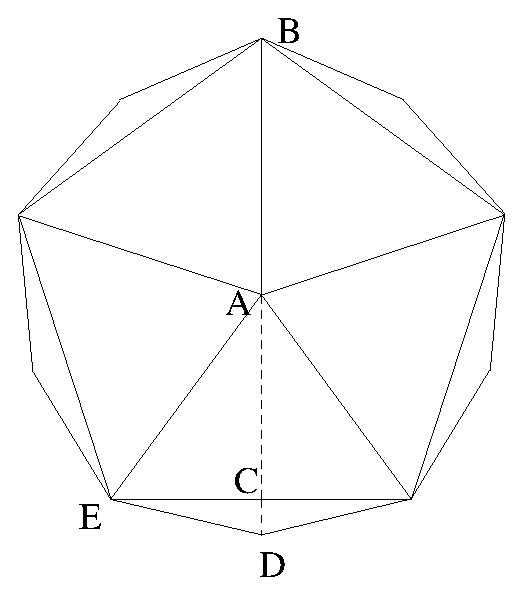
\includegraphics[clip,height=48mm,width=42mm]{1992math-3.eps}

\hspace{-10mm}図1
\end{center}
}\parbox[t]{80mm}{\hspace{-10mm}
\begin{center}
%
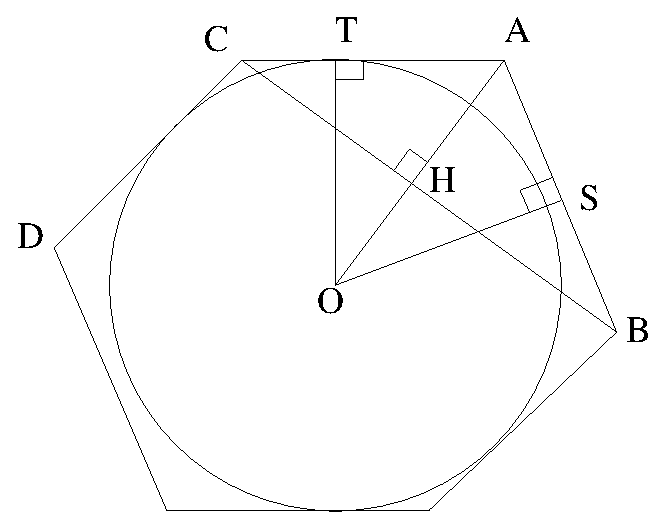
\includegraphics[clip,height=42mm,width=54mm]{1992math-4.eps}

図2
\end{center}
}

$ CE=\frac{a}{2} $より
\[
CH=CE\frac{1}{\tan\frac{\pi}{5}}=\frac{a}{2}\times\frac{\cos\frac{\pi}{5}}{\sqrt{1-\cos^2\frac{\pi}{5}}}
= \frac{a}{2}\sqrt{\frac{3+\sqrt{5}}{5-\sqrt{5}}}
\]

次に、図2で$\bigtriangleup$ACHにピタゴラスの定理を用いると
\[
AH^2+CH^2=AC^2
\]
\[
AH^2+\left(\frac{a}{2}\sqrt{\frac{3+\sqrt{5}}{5-\sqrt{5}}}
\right)^2=\left(\frac{\sqrt{3}}{2}a\right)^2 
\qquad \Yueni AH=\sqrt{\frac{3-\sqrt{5}}{5-\sqrt{5}}}  a
\]

ところで、図2で
$\bigtriangleup$ABHと$\bigtriangleup$AOSは相似より
\[
AO:AB=AS:AH  
\]

$\bigtriangleup$ACHと$\bigtriangleup$AOTは相似より
\[
AO:AC=OT:CH
\]

よって、
\begin{equation}
OT=\frac{AO \cdot CH}{AC} = \frac{AB \cdot AS \cdot CH}{AH \cdot AC}
 = a \frac{a}{2} \frac{a}{2} \sqrt{\frac{3+\sqrt{5}}{5-\sqrt{5}}}
 \sqrt{\frac{5-\sqrt{5}}{3-\sqrt{5}}} \frac{1}{a}
 \frac{2}{\sqrt{3}a}
 =  \frac{3\sqrt{3}+\sqrt{15}}{12} a
\eqname{radius}
\end{equation}

よって、内接球の半径$r=OT$は 
\[ r=\frac{3\sqrt{3}+\sqrt{15}}{12} a \]

また図2で再び$\bigtriangleup$ACHと$\bigtriangleup$AOTが相似であることに
注目すると
\[ AT:TO=AH:HC \qquad \Yueni AT=\frac{TO \cdot AH}{HC} \]
 
\eqhref{radius}より
\[ r=TO=\frac{AB \cdot AS \cdot CH}{AH \cdot AC} \]
であるから
\[
 AT =\frac{AB \cdot AS}{AC} 
    =a \frac{a}{2} \frac{2}{\sqrt{3}} \frac{1}{a} 
    = \frac{a}{\sqrt{3}} 
    = \frac{2}{3} AC
\]
したがって$T$、すなわち内接点は$AC$を$2:1$に内分する点、すなわち正三角形の面
の重心である。

\SubSubAnswer
正20面体はその対称性から、正三角形を底面とし、高さを内接球の半径と
する三角錐が20個あつまったもの、と考えられる。
三角錐の体積$v$は
\[
 v=\frac{1}{3} \left( \frac{1}{2} a \frac{\sqrt{3}}{2} a \right)
 \frac{3\sqrt{3}+\sqrt{15}}{12} a 
  = \frac{3+\sqrt{5}}{48} a^3
\]

したがって正20面体の体積$V$は
\[ V=20v=\frac{15+5\sqrt{5}}{12}a^3 \]
と求まる。

% 元の原稿ではここにも図1、図2を貼ってありました。
% 貼っても貼らなくてもどっちでもいいと思います。
\end{subsubanswers}
\end{subanswers}
\end{answer}




\end{document}



